\chapter{系统总体设计}

在深入探讨具体的硬件实现和软件编程细节之前,本章将阐述动态可重构矩阵乘法加速系统的整体架构。
系统设计遵循软硬件协同设计(Hardware/Software Co-design)的理念,旨在充分利用Xilinx Kria KV260平台的异构计算能力,
结合动态部分重构技术,实现一个既高性能又具备高度灵活性的矩阵运算加速解决方案。
本章将分别从硬件系统架构和软件系统架构两个层面进行阐述,为后续章节的详细实现奠定基础。

\section{硬件系统架构}

\subsection{设计总览}

\begin{figure}[htbp]
\centerline{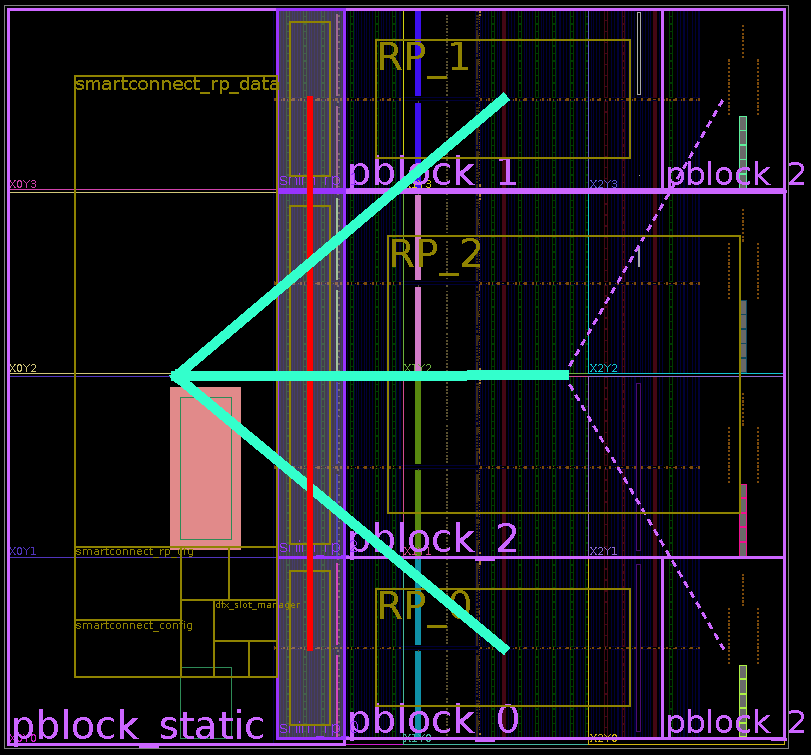
\includegraphics[width=0.8\columnwidth]{figures/synth.png}}
\caption{FPGA布局。RP\_0装载稀疏矩阵解压RM,RP\_1装载稀疏矩阵压缩RM,RP\_2装载稠密矩阵乘法RM。}
\label{fig:synth}
\end{figure}

\begin{table}[htbp]
\caption{FPGA资源分配}
\centering
\begin{tabular}{|l|c|c|c|c|}
\hline
\textbf{资源类型} & \textbf{静态区域} & \textbf{RP\_0} & \textbf{RP\_1} & \textbf{RP\_2}\\ \hline
LUT & 23040 & 19352 & 19352 & 54064 \\ \hline
FF & 46080 & 39360 & 39360 & 109440 \\ \hline
BRAM & 0 & 36 & 36 & 72 \\ \hline
DSP & 288 & 216 & 216 & 528 \\ \hline
\end{tabular}
\label{tab:resources}
\end{table}

如图\ref{fig:synth}所示,在FPGA的整体规划上,我们将其划分为左侧的静态区域(Static Region)和右侧的动态区域(Dynamic Region)。
表\ref{tab:resources}展示了分配给静态区域和3个RP的资源情况。
静态区域承载了系统运行所必需的基础逻辑,
例如与PS的接口控制器、时钟管理、中断管理等,以及连接RP的FIFO缓冲。本设计成功实现了三个独立的可重构分区(RP),
这三个分区为动态加载不同的计算模块提供了物理基础。每个可重构分区均设计为能够容纳一个可重构模块(RM)。
具体部署的RM包括稀疏矩阵解压模块、采用脉动阵列结合分块策略的稠密矩阵乘法模块以及稀疏矩阵压缩模块。
这些模块均采用Vitis高层次综合(HLS)语言编写,通过精心设计的pragma指令,实现了高度的并行计算和流水线操作,从而最大化地利用FPGA的硬件资源,提升运算效率。

\subsection{模块连接}

\begin{figure}[htbp]
\centerline{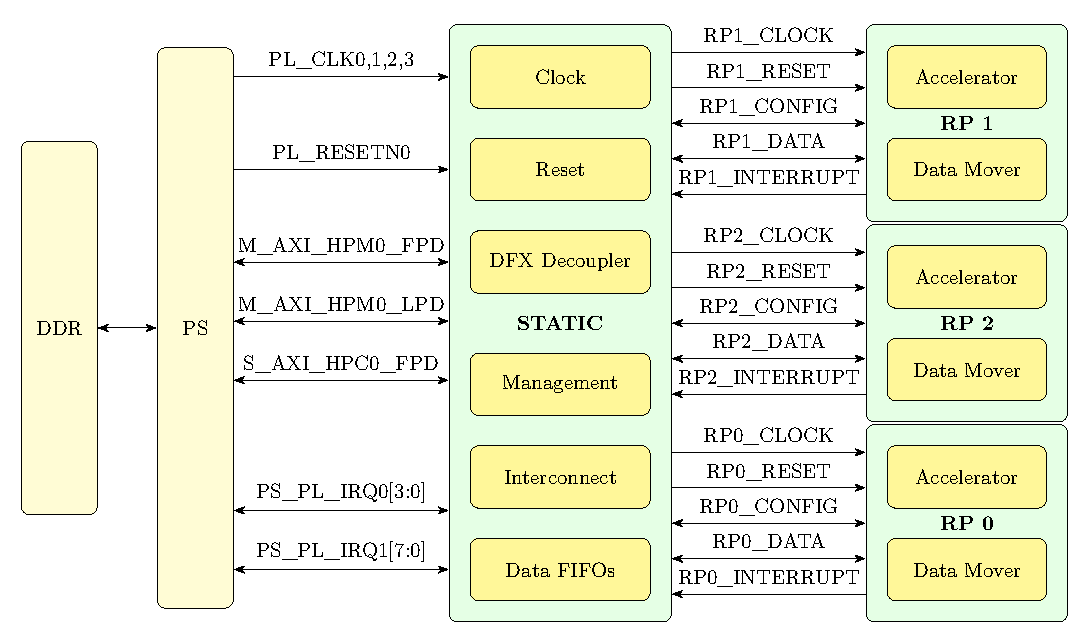
\includegraphics[width=0.8\columnwidth]{figures/arch.pdf}}
\caption{静态区域与动态区域间的连接。}
\label{fig:arch}
\end{figure}

\begin{figure}[htbp]
\centerline{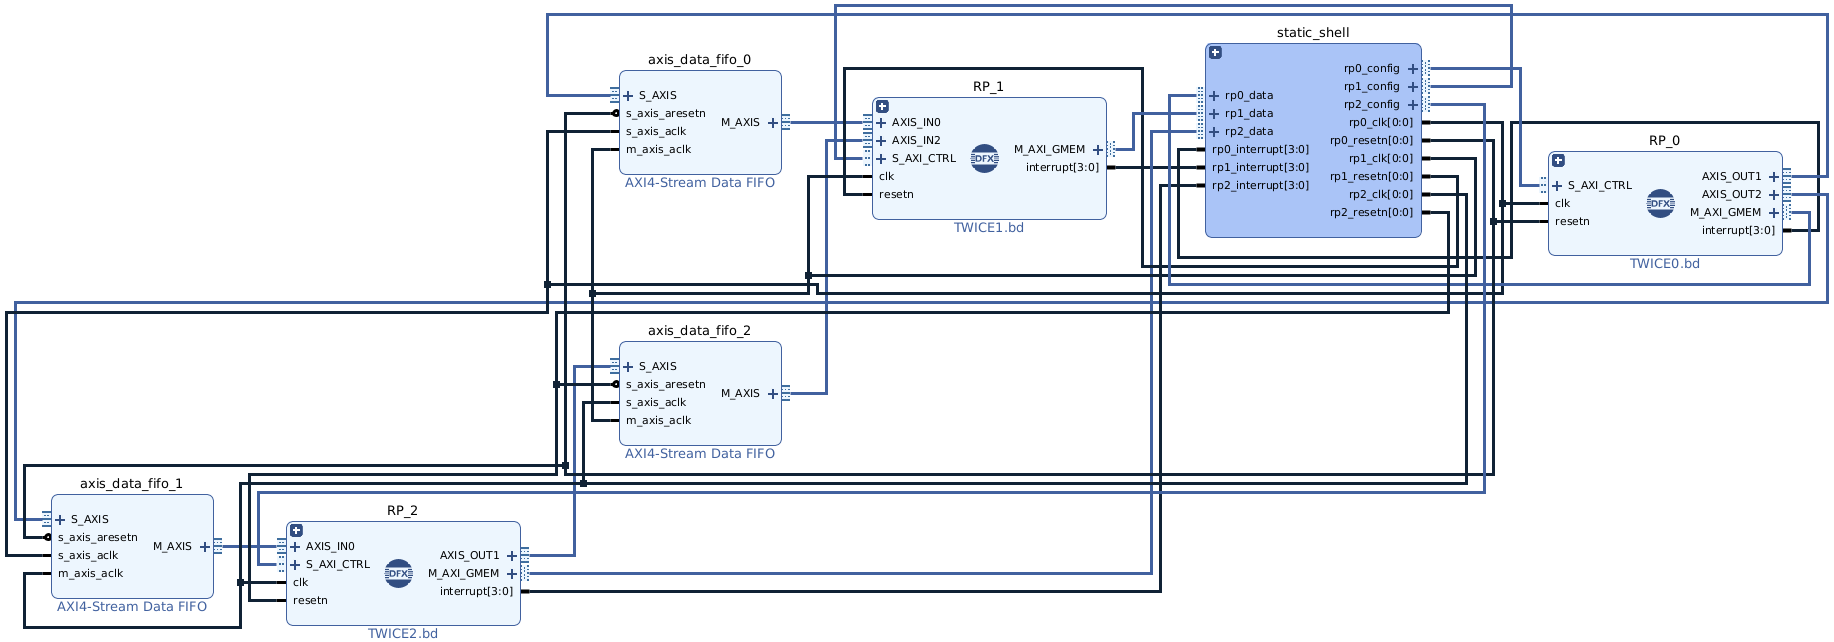
\includegraphics[width=\columnwidth]{figures/dfx.png}}
\caption{静态区域与RP间的连接,以及不同RP间的互联。}
\label{fig:dfx}
\end{figure}

\begin{figure}[htbp]
\centerline{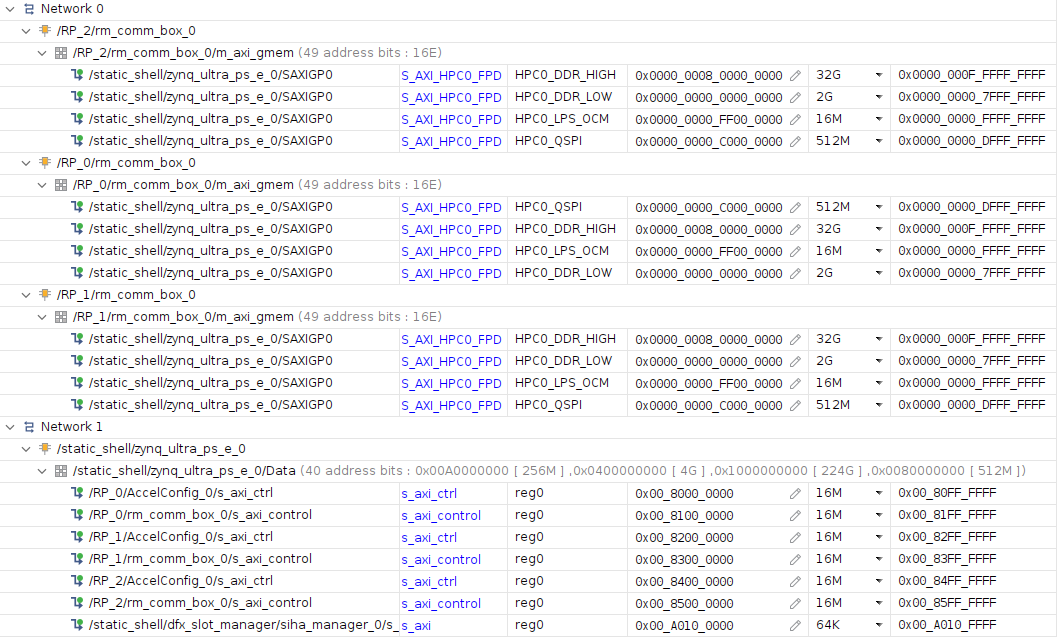
\includegraphics[width=0.8\columnwidth]{figures/mem.png}}
\caption{AXI地址空间分配。}
\label{fig:network}
\end{figure}

接口设计是确保数据高效流转和模块协同工作的关键。如图\ref{fig:arch}和图\ref{fig:dfx}所示,在可重构分区与KV260片上内存的交互方面,
采用了AXI4 Memory Mapped (AXIMM) 协议。这使得每个动态加载的RM都能够直接、
高效地对系统主存进行读写操作,为大规模矩阵数据的传输提供了高带宽通道。
静态区域与动态区域之间,以及动态区域与PS之间的控制与状态信号(CONFIG)交互,则通过AXI4 Lite接口实现。图\ref{fig:network}展示了为AXIMM与AXI Lite接口分配的地址空间。
同时,为了实现可重构模块之间的数据流传递和协同处理,例如将解压后的数据直接送入乘法模块,
我们设计了基于AXI4 Stream (AXIS) 协议的互联接口。这种流式接口非常适合于流水线式的处理流程,
能够有效减少数据在模块间传递的延迟。我们在RP间添加了数据缓冲队列,以实现更好的流水化。

\subsection{可重构分区}

\begin{figure}[htbp]
\centerline{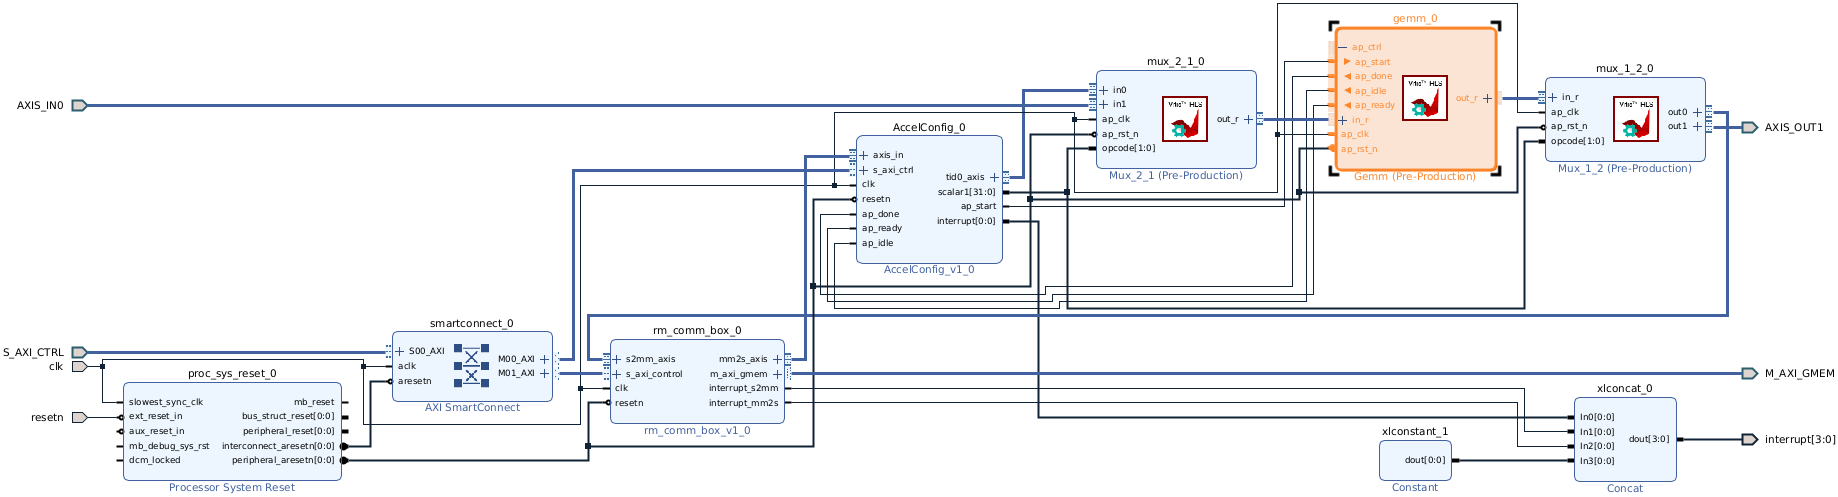
\includegraphics[width=\columnwidth]{figures/rp2.png}}
\caption{加载了稠密矩阵乘法RM(橙色高亮模块)的RP\_2内部设计。}
\label{fig:rp}
\end{figure}

图\ref{fig:rp}以稠密矩阵乘法的RP为例,展示了RP的内部结构。除了HLS编写的加速内核外,最重要的便是 \verb|rm_comm_box| 数据移动器IP核。
它具备用于从DDR/BRAM等存储器读写数据的AXIMM接口,一个为加速器提供输入的AXIS输出端口,以及一个用于从加速器读取数据的AXIS输入端口。
该IP核包含两个引擎:mm2s引擎通过AXIMM从内存地址读取数据,并将数据通过AXIS流输出端口提供出去;s2mm则是相反的步骤。

由于RP的输入/输出来源不确定,可能是DDR AXIMM也可能是其他RP的AXIS端口,我们编写了两个数据选择器。
数据选择器的控制信号通过 \verb|rm_comm_box| 提供的虚拟AXIS通道传输(由主机应用程序负责),这有别于其他AXI Lite传输的控制信号。

\section{软件系统架构}

软件系统架构是建立在KV260的ARM处理器之上,负责管理硬件资源、调度计算任务以及提供用户交互接口。
整个软件栈可以划分为操作系统层面、Xilinx运行时(XRT)应用层面以及顶层的任务调度逻辑。

在操作系统层面,KV260的CPU上部署了Ubuntu Linux操作系统。Linux系统为上层应用提供了稳定的运行环境和丰富的系统服务,
包括内存管理、进程调度以及设备驱动程序等。FPGA作为一种可编程设备,其驱动和管理由Linux内核模块以及Xilinx提供的运行时库共同完成。

XRT是连接用户空间应用程序与FPGA加速硬件之间的关键桥梁,提供了一套标准的API,
应用程序可以通过这些API来管理FPGA设备、分配和迁移数据缓冲区、加载FPGA比特流(包括用于动态重构的部分比特流)以及控制加速内核的执行。
在本系统中,我们编写的C/C++应用程序利用XRT提供的接口,实现了对FPGA上动态加载的矩阵运算模块的调用和管理,从而实现异构加速计算。
